\section{REVISÃO BIBLIOGRÁFICA}

\subsection{Mecânica dos Fluidos Aplicada à Engenharia de Poços de Petróleo}
	
Fluidos são substâncias capazes de escoar que se deformam com facilidade. Gases, líquidos e inclusive o plasma são classificados como fluidos. A mecânica dos fluidos está presente em uma vasta gama de situações: sistema respiratório e circulatório, esportes náuticos, bombas hidráulicas, ventiladores, turbinas, aviões, navios, rios, moinhos de vento, mísseis supersônicos, icebergs, motores, filtros, jatos e sprinklers. Quase tudo no mundo é um fluido ou se move dentro ou perto de um fluido \cite{White}. 
		
Os fluidos podem ser newtonianos ou não newtonianos. Fluido newtoniano é aquele que a viscosidade, ou atrito interno, é constante para diferentes taxas de cisalhamento. Nos fluidos newtonianos, a tensão é diretamente proporcional à taxa de deformação. Apesar de não existir um fluido perfeitamente newtoniano, fluidos considerados homogêneos, como a água e o ar, costumam ser estudados como newtonianos para muitas finalidades práticas \cite{Pordeus}.
		
		
Fluido não-newtoniano é aquele cuja viscosidade varia proporcionalmente à energia cinética que se imprime a esse mesmo fluido, respondendo de forma quase instantânea. Para exemplo temos a mistura do amido de milho com água que, dependendo da pressão que recebe, pode ser um sólido ou um líquido, apresentando característica viscosa. Com pressão suficiente, torna-se um sólido e com menor pressão volta ao estado líquido \cite{Pordeus}.
		
		
Outra característica de um fluido diz respeito à sua compressibilidade. Um fluido \emph{compressível} é aquele que possui a habilidade de ser comprimido em um recipiente quando seu volume diminui por ação de uma força aplicada. A massa específica do fluido muda em relação ao grau de compressão sofrido . Já um fluido \textit{incompressível} é aquele cuja massa específica permanece relativamente constante, ou seja, que resiste à redução de seu volume quando submetido a uma força compressiva \cite{Pordeus}.
		
\subsubsection{Colchões}

Para que haja remoção eficiente do fluido de perfuração na parede da formação no interior dos poços de petróleo, são injetados fluidos denominados colchões lavadores e colchões espaçadores antes da pasta de cimento, como dito anteriormente. Estes colchões têm distintas finalidades durante o processo de limpeza do poço.
			
Colchão lavador é um fluido com baixa viscosidade e baixa massa específica compatível com o fluido de perfuração. Por meio de ações químicas e mecânicas, ele dilui e remove o reboco (camada de baixa permeabilidade formado pelos fluidos de perfuração nas paredes do poço).

Colchão espaçador é, geralmente, um fluido com viscosidade e massa específica altas que atua apenas de forma mecânica para a remoção do reboco. Semelhantemente aos colchões lavadores, também são injetados antes da pasta de cimento com o intuito de evitar o contato dela com o fluido de perfuração. Eles ajudam a preservar eventuais problemas de cimentação, a exemplo da formação de canais de fluido no interior do cimento que prejudicam o isolamento hidráulico \cite{Campos}.
			
A Fig. \ref{fig:remocao_fluido} ilustra o funcionamento dos colchões na engenharia de poços. Podemos observar que o colchão lavador (cor azul clara), depois de injetado pelo interior do revestimento, retorna à superfície pelo espaço anular empurrando o fluido de perfuração responsável pelo carreamento de detritos (cor marrom). Em seguida, o colchão espaçador (cor verde), remove o restante dos fluidos anteriormente injetados para que a pasta de cimento (cor cinza) se adira às paredes da formação adequadamente \cite{Campos}.
\begin{figure}[H]
    \centering
    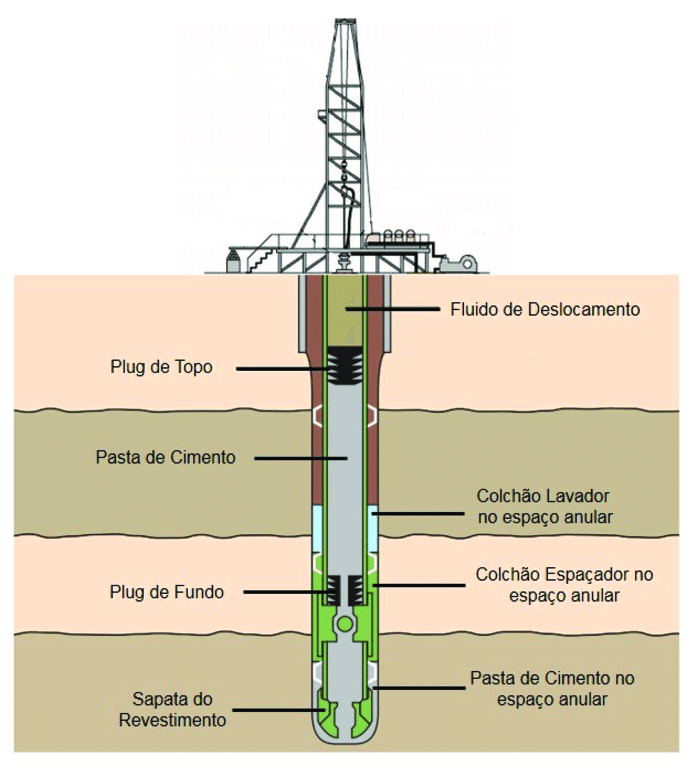
\includegraphics[scale=0.35]{img/remocao_fluido.png}
    \caption
    [Remoção de fluido de perfuração por ação de colchões (lavador e espaçador) durante a cimentação primária de um poço de petróleo.]
    {Remoção de fluido de perfuração por ação de colchões (lavador e espaçador) durante a cimentação primária de um poço de petróleo. Fonte: \cite{Curbelo}.}
    \label{fig:remocao_fluido}
\end{figure}
		
	
\subsubsection{Excentricidade do Tubo de Revestimento}

Quando o eixo do tubo de revestimento (\textit{casing}) coincide com o eixo do poço perfurado, diz-se que o arranjo está sob uma configuração anular concêntrica. Neste caso, os fluidos deslocam-se no espaço anular de maneira relativamente simétrica, proporcionando aos processos de limpeza e cimentação certo grau de uniformidade na parede do poço. Entretanto, quando o tubo de revestimento está deslocado do centro, a configuração do anular torna-se excêntrica, os colchões tendem a fluir de maneira não uniforme. A presença de excentricidade (\textit{standoff}) no tubo de revestimento é um fator que influencia fortemente o deslocamento de fluidos durante os processos de perfuração e completação de poços de petróleo.

O comprometimento da eficiência de varredura pode ocorrer com qualquer fluido injetado, inclusive com a pasta de cimento. Em geral, para que não haja pontos da formação com lacunas de cimentação, centralizadores são instalados no tubo para manter o espaço anular o mais uniforme possível. 
A excentricidade entre poço e revestimento é medida, em geral, por um parâmetro popularmente conhecido como \textit{standoff}. A taxa de standoff pode ser representada por um percentual que varia entre 0\% (revestimento em contato com a parede) e 100\% (revestimento afastado ao máximo da parede). Entretanto, os limites inferior e máximo são praticamente inatingíveis, permanecendo a taxa em valores intermediários. 
Obter valores genuinamente altos de \textit{standoff} é uma tarefa extremamente difícil para a engenharia de poços. Além disso, o próprio revestimento pode dobrar ou ceder em alguns pontos no interstício entre um centralizador e outro, resultando em um \textit{standoff} notadamente menor (\textit{sag point}). Por isso, durante o trabalho de limpeza, o colchão lavador encontrará maior resistência para deslocar o fluido de perfuração na porção anular que estiver espremida, deixando para trás resquícios de detritos não carreados. Um exemplo desse problema é mostrado na Fig. \ref{fig:Standoff1}, relativo a um incidente ocorrido com o poço de Macondo, no Golfo do México, em 2011 
\cite{Macondo,Hanieh}.
\begin{figure}[H]
	\centering
	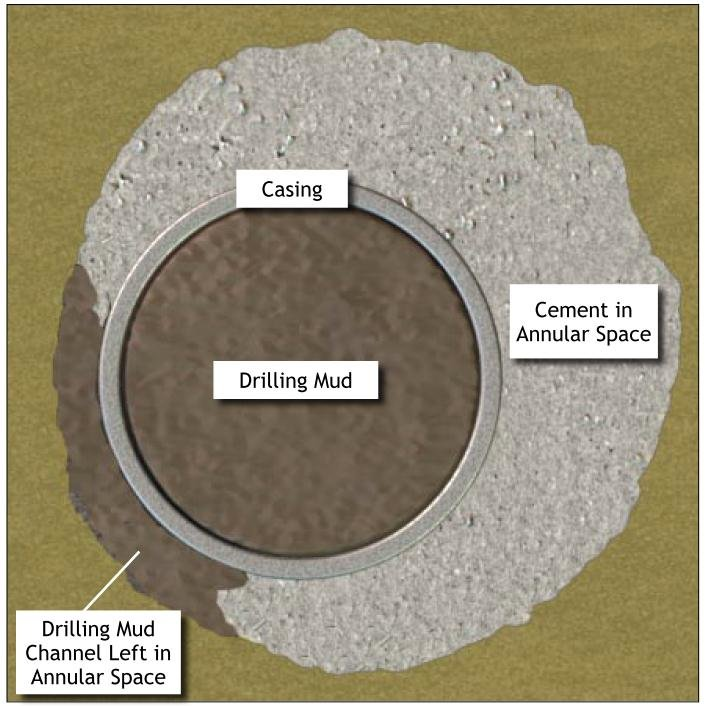
\includegraphics[scale=0.7]{img/Standoff1.png}
	\caption[Seção transversal de um revestimento excêntrico.]{Seção transversal de um revestimento excêntrico.}
	\label{fig:Standoff1}
\end{figure}
A Fig. \ref{fig:Standoff2} mostra um caso de \textit{standoff} menor entre dois centralizadores \cite{VADIM}.
\begin{figure}[H]
	\centering
	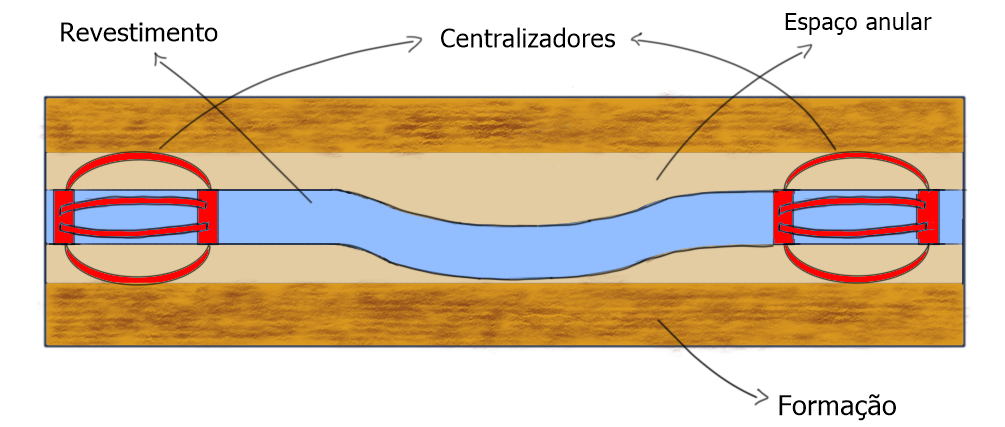
\includegraphics[width=0.7\linewidth]{img/centralizadores_standoff.png}
	\caption[\textit{Standoff} menor do que 100\% entre dois centralizadores.]{\textit{Standoff} menor do que 100\% entre dois centralizadores. Fonte: autor.}
	\label{fig:Standoff2}
\end{figure}

Considerando a seção transversal de um anel excêntrico, como se vê na Fig. \ref{fig:secao_transversal_equivalente_livro}, a taxa de \textit{standoff} pode ser calculada como \cite{Erik}: 
\begin{equation}
    \varsigma = (1 - \alpha) 100\%, \quad \text{com} \quad \alpha = \frac{e}{r_o - r_i},
\end{equation}
onde $e$ é a distância entre o centro do poço e o centro do tubo de revestimento, $r_o$ é o raio do poço e $r_i$ é o raio do tubo de revestimento. O cálculo do \textit{standoff} usa um ponto de referência na parede do poço para definir o afastamento, especificamente na interseção inferior que se acha entre a circunferência do poço aberto e a linha de simetria que passa pelo ângulo desdobrado de $\pi$ radianos (Fig. \ref{fig:secao_transversal_equivalente_livro}). Dessa forma, $\varsigma = 0\%$ equivale a dizer que o revestimento toca a parede do poço no tal ponto, enquanto que $\varsigma = 100\%$ equivale a dizer que o revestimento dista o máximo possível desse ponto. Em outras palavras, $\varsigma = 100\%$ significaria concentricidade ``perfeita''.
\begin{figure}[H]
	\centering
	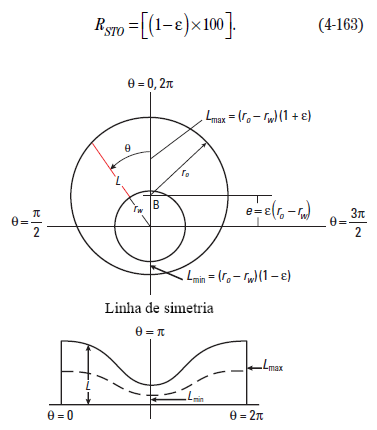
\includegraphics[width=0.75\linewidth]{img/Standoff_livro_Well.png}
	\caption{Seção transversal equivalente a um revestimento excêntrico. Fonte: \cite{Erik}}
	\label{fig:secao_transversal_equivalente_livro}
\end{figure}
Neste trabalho, consideramos simulações em que $0\% < \varsigma \leq 100\%$. Em particular, o caso em que $\varsigma$ é máximo é utilizado como modelo ideal de referência.

\subsection{Objetivos de Pesquisa}

A Matemática Computacional é capaz de propor modelos matemáticos para resolver problemas reais de alta complexidade. Aqui, procuramos dar enfoque à melhoria de processos industriais relacionados à perfuração de poços de petróleo, um tema interdisciplinar que integra diversas áreas de conhecimento, tais como matemática, física, computação e as engenharias química, mecânica e de petróleo. 

Estudar o comportamento do escoamento de colchões lavadores e sua eficiência de limpeza em diferentes configurações de poços traz benefícios para o desenvolvimento científico e tecnológico nacional, além de motivar talentos para a pesquisa. A seguir, destacamos os principais objetivos estabelecidos para a pesquisa.

\subsubsection{Objetivo Geral}

Simular numericamente o escoamento de colchões lavadores caracterizados por propriedades constituintes similares às de óleos biodegradáveis não inflamáveis que se desenvolvem durante a etapa de pré-cimentação de poços de petróleo.

\subsubsection{Objetivos Específicos}

\begin{itemize}
	\item Aplicar o método dos elementos finitos para solucionar numericamente as equações de Navier-Stokes para fluidos incompressíveis;
	\item Implementar códigos computacionais tomando como base a biblioteca FEniCS;
	\item Gerar malhas numéricas para diferentes características geométricas de poço e de espaço anular, simulando efeitos de erosão e excentricidade (\textit{standoff});
	\item Definir um parâmetro para quantificar a eficiência de varredura do escoamento em regime laminar;
	\item Analisar resultados de simulação para configurações de poço bidimensionais;
\end{itemize}

